\section{Quantum Walks}
\label{sec:quantum_walk}

\subsection{Quantum Walk on a Line}
\label{subsec:quantum_walk_line}

%proofed
Quantum Walk is the quantum version of random walks, which are mathematical formalisms that describe a path composed of random steps. A Markov Chain might be used to describe these processes.

We can define the Discrete Quantum Walk on a Line as a series of Left/Right decisions. Understanding this algorithm is important towards being able to define and design more complex algorithms that make use of quantum properties.

%proofed
 
%spelling 4; punctuation 3 weak

We followed an approach suggested by \cite{Ambainis} towards simulating n-steps of a Quantum Walk on a Line. The algorithm can be consulted on \ref{ap:a}.
In a discrete quantum walk in a line we want to preserve the fact that the probability of turning left is equal to the probability of turning right.  To represent a state in this algorithm we will need the number of the node and a direction (identified as L,R) \ref{eq:3_qwl_state}.

%spelling 4; punctuation 3 weak

\begin{equation}
\label{eq:3_qwl_state}
\vert \psi\rangle = \vert n, L\rangle
\end{equation}

With two equally possible direction choices in each step, we can use a coin metaphor\cite{Ambainis}\cite{Ambainis2008} to approach the decision. We toss a coin and go either Left or Right depending on the result. 

In a quantum version we need to define a Coin Operator (Coin Matrix), which is responsible to imprint a direction to the current state. This operator is a unitary matrix in a 2-dimension Hilbert space. Some examples of Coin Operators are the Hadamard matrix\ref{eq:hadamard} and a symmetric unitary matrix \ref{eq:qwl_symmetric}.

\begin{equation}
\label{eq:hadamard}
H=\frac{1}{\sqrt{2}}\left[\begin{array}{cc}
1 & 1\\
1 & -1
\end{array}\right]
\end{equation}

\begin{equation}
\label{eq:qwl_symmetric}
\left[\begin{array}{cc}
\frac{1}{\sqrt{2}} & \frac{i}{\sqrt{2}}\\
\frac{i}{\sqrt{2}} & \frac{1}{\sqrt{2}}
\end{array}\right]
\end{equation}

Taking the Hadamard matrix as an example\ref{eq:hadamard}, the coin matrix will operate on the state in the following way \ref{eq:qwl_1}\ref{eq:qwl_2}\cite{Ambainis}.

\begin{equation}
\label{eq:qwl_1}
C\vert n, L\rangle = \frac{1}{\sqrt{2}} \vert n, L\rangle + \frac{1}{\sqrt{2}} \vert n, R\rangle
\end{equation}
  
\begin{equation}
\label{eq:qwl_2}
C\vert n, R\rangle = \frac{1}{\sqrt{2}} \vert n, L\rangle - \frac{1}{\sqrt{2}} \vert n, R\rangle
\end{equation} 

The Coin Matrix obtains its name by being the quantum equivalent of flipping a classic coin. After tossing a coin comes an operator that will move the node in the direction assigned. The operator responsible for this modification is commonly referred as Shift Operator \ref{eq:qwl_3}\ref{eq:qwl_4}. 

\begin{equation}
\label{eq:qwl_3}
S\vert n, L\rangle = \frac{1}{\sqrt{2}} \vert n-1, L\rangle
\end{equation}

\begin{equation}
\label{eq:qwl_4}
S\vert n, R\rangle = \frac{1}{\sqrt{2}} \vert n+1, R\rangle
\end{equation} 

These matrices (Coin Matrix and Shift Operator) are referred conceptually ubiquitously throughout the literature \cite{SAUCES}, therefore it is important to be familiar with them. A single step of the algorithm \ref{ap:a} is illustrated in Figure \ref{fig:qwl_tree}.

[needs more explaining]

\begin{figure}[h]
\centering 

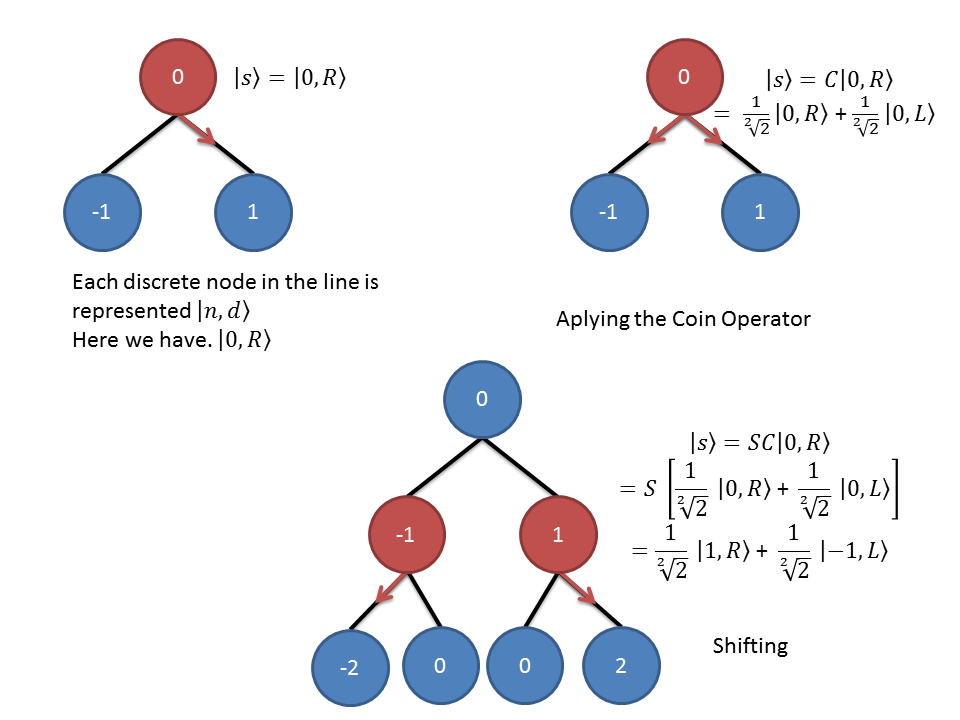
\includegraphics[scale=0.50]{Figures/quantum_walk_line.png}
\caption{Simulating a step of a discrete quantum walk on a line. In the beginning we have a state characterized by the position $(0)$ and a direction (either Left or Right).}
\label{fig:qwl_tree}
\end{figure}


Depending on the Coin Matrix we can get different distributions. In Figures \ref{fig:qwl_hadamard} and \ref{fig:qwl_symetric}

\begin{figure}[h]
\centering 
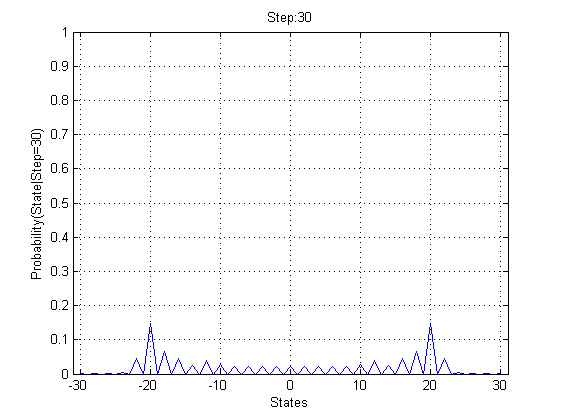
\includegraphics[scale=0.50]{Figures/quantum_walk_line_symetric.png}
\caption{30 Step of the Simulation \ref{ap:a} using Matrix \ref{eq:hadamard} as a Coin Operator.}
\label{fig:qwl_symetric}
\end{figure}

\begin{figure}[h]
\centering 
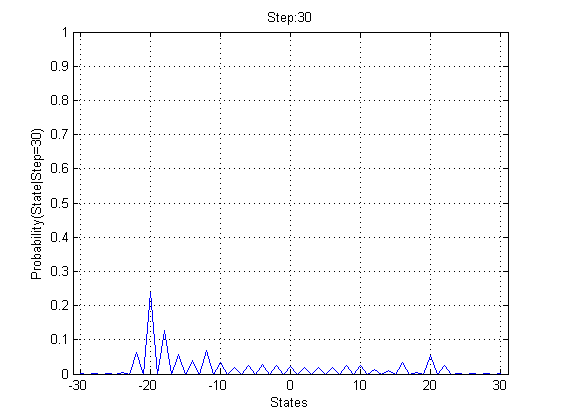
\includegraphics[scale=0.50]{Figures/quantum_walk_line_hadamard.png}
\caption{30 Step of the Simulation \ref{ap:a} using a Hadamard Matrix \ref{eq:hadamard} as a Coin Operator.}
\label{fig:qwl_hadamard}
\end{figure}

Starting on the middle of a line we can shift one unit left or right.
If we took the classical approach in which we tossed a fair coin, and after n-steps we measured the final node repeatedly, by the \ac{CLT} the final distribution would converge to a normal distribution.

\subsection{Quantum Walk on a Line}
\label{subsec:quantum_walk_line}
